\documentclass[aspectratio=169,11pt]{beamer}
\usepackage[utf8]{inputenc}
\DeclareUnicodeCharacter{21D2}{$\Rightarrow$}
\DeclareUnicodeCharacter{2080}{$_0$}
\DeclareUnicodeCharacter{2264}{$\leq$}
\DeclareUnicodeCharacter{2265}{$\geq$}
\DeclareUnicodeCharacter{2260}{$\neq$}
\DeclareUnicodeCharacter{2192}{$\to$}
\DeclareUnicodeCharacter{211D}{$\mathbb{R}$}
\DeclareUnicodeCharacter{03B3}{$\gamma$}
\DeclareUnicodeCharacter{03C3}{$\sigma$}
\DeclareUnicodeCharacter{03B5}{$\varepsilon$}
\DeclareUnicodeCharacter{039B}{$\Lambda$}
\DeclareUnicodeCharacter{03C9}{$\omega$}
\usepackage[T1]{fontenc}
\usepackage[english]{babel}
\usepackage{amsmath,amssymb}
\usepackage{booktabs}
\usepackage{graphicx}
\usepackage{listings}
\usetheme{default}
\usecolortheme{seahorse}
\setbeamertemplate{navigation symbols}{}
\setbeamertemplate{footline}[frame number]
\setbeamerfont{frametitle}{size=\large}

\lstdefinelanguage{Lean}{
  morekeywords={theorem,lemma,def,noncomputable,by,intro,apply,exact,have,rw,simp,simpa,only,
    linarith,nlinarith,show,fun,let,Prop,refine,constructor,rcases,with,at,ring,field_simp,
    HasDerivAt,StrictMono,using,set},
  sensitive=true,
  morecomment=[l]{--},
  morecomment=[s]{/-}{-/},
}
\lstset{
  language=Lean,
  basicstyle=\ttfamily\scriptsize,
  keywordstyle=\color{blue!70!black}\bfseries,
  commentstyle=\color{gray},
  columns=fullflexible,
  keepspaces=true,
  breaklines=true,
  extendedchars=true,
  inputencoding=utf8,
  literate=
    {∀}{{$\forall$}}1 {∃}{{$\exists$}}1 {ℝ}{{$\mathbb{R}$}}1 {→}{{$\to$}}1 {↔}{{$\leftrightarrow$}}1
    {∈}{{$\in$}}1 {≤}{{$\leq$}}1 {≥}{{$\geq$}}1 {≠}{{$\neq$}}1 {⟨}{{$\langle$}}1 {⟩}{{$\rangle$}}1
    {₀}{{$_0$}}1 {¬}{{$\neg$}}1 {∧}{{$\wedge$}}1 {∨}{{$\vee$}}1 {·}{{$\cdot$}}1 {⇒}{{$\Rightarrow$}}1
    {←}{{$\leftarrow$}}1 {γ}{{$\gamma$}}1 {σ}{{$\sigma$}}1 {ε}{{$\varepsilon$}}1 {Λ}{{$\Lambda$}}1
    {⁻¹}{{$^{-1}$}}2
}

\title{Acemoglu \& Restrepo (2018)}
\subtitle{\emph{The Race between Man and Machine} --- displacement, reinstatement, and the condition under which automation raises wages}
\author{Manuel Arriola}
\date{Repository 6 \textperiodcentered{} Week of September 21 -- 26, 2026}

\begin{document}

%================= PORTADA =============================================
\begin{frame}[plain]
  \titlepage
  \begin{center}\small
    \texttt{github.com/Arriola123456/ai-06-restrepo}\\[2pt]
    \footnotesize Version read: NBER Working Paper 22252 as revised in June 2017 (87 pp., the course PDF; title
    \emph{The Race Between Machine and Man}), pinned by SHA-256 in \texttt{lean/}. Page numbers are the PDF's
    (printed page $=$ PDF page $-2$). Backup slides after slide 14.
  \end{center}
\end{frame}

%================= 1. EL PAPER Y EL PROBLEMA =========================
\begin{frame}{1 \textperiodcentered{} The paper and the problem: the unit of analysis is the economy}
  \footnotesize
  \textbf{Question.} Technology enters as \emph{automation} (machines take over tasks previously done by
  labor) and as \emph{new tasks} (labor gets new things to do). What does each do to output, wages, the labor
  share and employment --- and can the economy keep a stable labor share when both run at once?

  \smallskip
  \textbf{This is the only paper of the term whose agent is the aggregate economy.} There is no individual
  optimising over a menu of AI tools: there is a unit measure of tasks $i\in[N-1,N]$, competitive firms that
  pick the cheaper factor for each task, a representative household supplying labor, and a capital stock $K$.
  The ``problem'' is a competitive equilibrium, and the objects that move are $I$ (how far automation has
  reached) and $N$ (how far the task frontier has moved).

  \smallskip
  \textbf{Environment (Section 2.1, p.\ 8--9).} Final good $Y=\tilde B\big(\int_{N-1}^N y(i)^{\frac{\sigma-1}{\sigma}}di\big)^{\frac{\sigma}{\sigma-1}}$.
  Tasks $i\le I$ are technologically automated: capital and labor are perfect substitutes there,
  $k(i)+\gamma(i)l(i)$; tasks $i>I$ need labor with productivity $\gamma(i)$.
  \textbf{Assumption 1:} $\gamma$ strictly increasing --- labor's comparative advantage rises with the task index.
  Preferences $u(C,L)$ with an increasing labor supply $L=L^s(\omega)$, $\omega=W/(RK)$ (eq.\ 11).
  \textbf{Assumption 2:} homothetic demand ($\eta\to0$ or $\zeta=1$), so $\hat\sigma=\sigma(1-\eta)+\zeta\eta$ is the
  elasticity between capital and labor. \textbf{Assumption 3:} $K<\underline K$, i.e.\ $R>W/\gamma(N)$: new tasks
  are adopted at once.
\end{frame}

\begin{frame}{1 \textperiodcentered{} The threshold: who does which task (p.\ 10)}
  \footnotesize
  Tasks are priced at minimum unit cost,
  \[
    p(i)=\begin{cases}\min\{R,\,W/\gamma(i)\}^{1-\eta} & i\le I\\ (W/\gamma(i))^{1-\eta} & i>I.\end{cases}
  \]
  Since $\gamma$ is increasing there is a unique $\tilde I$ with $\dfrac{W}{R}=\gamma(\tilde I)$ (eq.\ 6): capital
  is cheaper below it, labor above it. Technology may bind before cost does, so the equilibrium threshold is
  \[
    I^*=\min\{I,\tilde I\}:\qquad i<I^*\ \text{produced with capital},\qquad i>I^*\ \text{with labor}.
  \]
  Two regimes run through everything that follows:
  \begin{itemize}
    \item \textbf{technology-constrained}, $I^*=I<\tilde I$: firms would automate more if they could;
    \item \textbf{cost-minimising}, $I^*=\tilde I<I$: the frontier is slack; factor prices decide.
  \end{itemize}
  \textbf{Proposition 1 (p.\ 12).} Unique equilibrium; output is a CES aggregate with endogenous shares,
  \[
    Y=\tfrac{B}{1-\eta}\Big[(I^*-N+1)^{\frac1{\hat\sigma}}K^{\frac{\hat\sigma-1}{\hat\sigma}}
      +\Big(\textstyle\int_{I^*}^N\gamma(i)^{\hat\sigma-1}di\Big)^{\frac1{\hat\sigma}}L^{\frac{\hat\sigma-1}{\hat\sigma}}\Big]^{\frac{\hat\sigma}{\hat\sigma-1}},
  \]
  and $\omega$ solves the relative demand (13). \textbf{Corollary 1:} with $\sigma=\zeta=1$, $\gamma\equiv1$,
  $Y=\frac{B}{1-\eta}K^{1-N+I^*}L^{N-I^*}$: the labor share \emph{is} $N-I^*$.
\end{frame}

%================= 2. RESULTADO PRINCIPAL ============================
\begin{frame}{2 \textperiodcentered{} The main result I: Proposition 2, the two forces are polar (p.\ 11)}
  \footnotesize
  Let $\varepsilon_L>0$ be the labor-supply elasticity and
  $\Lambda_I=\dfrac{\gamma(I^*)^{\hat\sigma-1}}{\int_{I^*}^N\gamma^{\hat\sigma-1}}+\dfrac1{I^*-N+1}>0$,
  $\Lambda_N=\dfrac{\gamma(N)^{\hat\sigma-1}}{\int_{I^*}^N\gamma^{\hat\sigma-1}}+\dfrac1{I^*-N+1}>0$.

  \textbf{Technology-constrained case ($I^*=I<\tilde I$):}
  \[
    \frac{d\ln(W/R)}{dI}=-\frac{\Lambda_I}{\hat\sigma+\varepsilon_L}<0,\qquad
    \frac{d\ln(W/R)}{dN}=\frac{\Lambda_N}{\hat\sigma+\varepsilon_L}>0,\qquad
    \frac{d\ln(W/R)}{d\ln K}=\frac{1+\varepsilon_L}{\hat\sigma+\varepsilon_L}>0.
  \]
  \textbf{Cost-minimising case ($I^*=\tilde I<I$):} $d\ln(W/R)/dI=0$ and
  $d\ln(W/R)/dN=\Lambda_N/(\sigma_{free}+\varepsilon_L)>0$ with $\sigma_{free}=\hat\sigma+\Lambda_I/\varepsilon_\gamma>\hat\sigma$.

  \smallskip
  \textbf{In all cases} the labor share and employment move with $\omega$: $dL/dN>0$, and when $I^*=I$,
  $dL/dI<0$. So automation is always capital-biased (lowers $W/R$, $s_L$, $L$) and new tasks are always
  labor-biased (raise all three) --- \emph{displacement} against \emph{reinstatement}.
\end{frame}

\begin{frame}{2 \textperiodcentered{} The main result II: Proposition 3, the wage is the ambiguous object (p.\ 13)}
  \footnotesize
  Constrained case, with $W/\gamma(I^*)>R>W/\gamma(N)$:
  \[
    d\ln Y|_{K,L}=\underbrace{\tfrac{B^{\hat\sigma-1}}{1-\hat\sigma}\Big(\big(\tfrac{W}{\gamma(I^*)}\big)^{1-\hat\sigma}-R^{1-\hat\sigma}\Big)}_{\text{productivity effect of automation}\ >0}dI
    +\tfrac{B^{\hat\sigma-1}}{1-\hat\sigma}\Big(R^{1-\hat\sigma}-\big(\tfrac{W}{\gamma(N)}\big)^{1-\hat\sigma}\Big)dN,
  \]
  \[
    d\ln W=d\ln Y|_{K,L}+(1-s_L)\Big(\tfrac{\Lambda_N}{\hat\sigma+\varepsilon_L}dN-\underbrace{\tfrac{\Lambda_I}{\hat\sigma+\varepsilon_L}dI}_{\text{displacement}}\Big),\qquad
    d\ln R=d\ln Y|_{K,L}-s_L\Big(\tfrac{\Lambda_N}{\hat\sigma+\varepsilon_L}dN-\tfrac{\Lambda_I}{\hat\sigma+\varepsilon_L}dI\Big).
  \]
  New tasks always raise $W$; automation always raises $R$ and \textbf{raises $W$ iff the productivity effect
  exceeds the displacement effect}. The productivity effect is the cost saving $W/\gamma(I^*)-R$ on the
  marginal automated task; the displacement effect is $(1-s_L)\Lambda_I/(\hat\sigma+\varepsilon_L)$.
  Cost-minimising case: automation does nothing to factor prices; new tasks raise $W$ and may lower $R$.

  \smallskip
  \textbf{Conditions, spelled out.} Assumptions 1--3; $\hat\sigma\neq1$ in the displayed productivity term
  (Cobb-Douglas is the limit); $K$ fixed (static); the sign of $d\ln W/dI$ depends on $K$ --- next slide.
\end{frame}

\begin{frame}{2 \textperiodcentered{} The trap: ``does automation necessarily reduce wages and the labour share?''}
  \footnotesize
  \begin{center}\scriptsize
  \begin{tabular}{@{}llll@{}}
    \toprule
    & $I\uparrow$, constrained & $I\uparrow$, cost-min. & $N\uparrow$\\
    \midrule
    $W/R$, $s_L$, $L$ & fall, always (Prop.\ 2) & unchanged & rise, always\\
    $R$ & rises, always (Prop.\ 3) & unchanged & may fall\\
    $W$ & \textbf{ambiguous}: productivity vs displacement & unchanged & rises, always\\
    $Y|_{K,L}$ & rises & unchanged & rises\\
    \bottomrule
  \end{tabular}
  \end{center}
  \textbf{Flat answer:} ``yes, automation lowers wages and the labor share.'' \textbf{Paper:} the labor share, yes,
  always (when technology binds); the wage, no --- it rises when the cost saving on the marginal task is large.

  \smallskip
  \textbf{The condition, in closed form (Corollary 1, my derivation, proved in Lean):} with
  $Y=cK^{1-s}L^{s}$, $s=N-I^*$, $\ \ln W=\ln c+\ln s+(1-s)\ln K+(s-1)\ln L$, so
  \[
    \frac{d\ln W}{dI^*}=\ln\frac KL-\frac1{N-I^*}>0\iff \frac KL>e^{1/(N-I^*)}=:\frac{\bar K}{L}.
  \]
  Automation raises the wage when capital is \emph{abundant} enough --- $R$ low, the saving $W-R$ large. And
  $\bar K/L=e^{1/s}>\underline K/L=(1-s)/s$: inside Assumption 3 ($K<\underline K$) the wage always falls.
  \textbf{Proposition 3 prints the opposite direction} (``increases the wage when $K<\bar K$''); slide 12.
\end{frame}

%================= 3. LO QUE HICE ====================================
\begin{frame}{3 \textperiodcentered{} What I did analytically and computationally}
  \footnotesize
  \begin{itemize}
    \item \textbf{By hand} (\texttt{hand/}, slide 13): the cost threshold and $I^*$; the Cobb-Douglas case ---
      $W$, $R$, $s_L=N-I^*$ and the sign of $d\ln W/dI^*$.
    \item \textbf{Numerics} (\texttt{analysis/task\_model.py}): the static equilibrium of Section 2 solved from
      eq.\ (13) with $\gamma(i)=0.3e^{3i}$, $\hat\sigma=0.6$, $\varepsilon_L=0.3$, $L^s(\omega)=\omega^{\varepsilon_L}$;
      the two regimes detected from $W/R\gtrless\gamma(I)$; prices from the ideal price index (10).
    \item \textbf{Check against the paper:} the numerical total derivative $d\ln W/dI$ equals Proposition 3's
      formula (productivity minus displacement) to four decimals at every point tried.
    \item \textbf{Findings:} $s_L$ and $L$ fall with $I$ everywhere; $W$ falls throughout the Assumption-3
      window ($K<\underline K=4.73$ at $I=0.5$) and rises only beyond $\bar K=5.73>\underline K$; new tasks raise
      $W$ and $s_L$; the closed-form Cobb-Douglas threshold $\bar K/L=e^{1/(N-I^*)}$ matches.
    \item \textbf{Lean via AppliedModelingLib} (slides 10--12): ten source-facing statements of Section 2 proved;
      the Cobb-Douglas wage response as an extension. Status partially formalized.
  \end{itemize}
\end{frame}

\begin{frame}{3 \textperiodcentered{} Automation: $s_L$ and $L$ always fall, $W$ may go either way}
  \begin{center}
    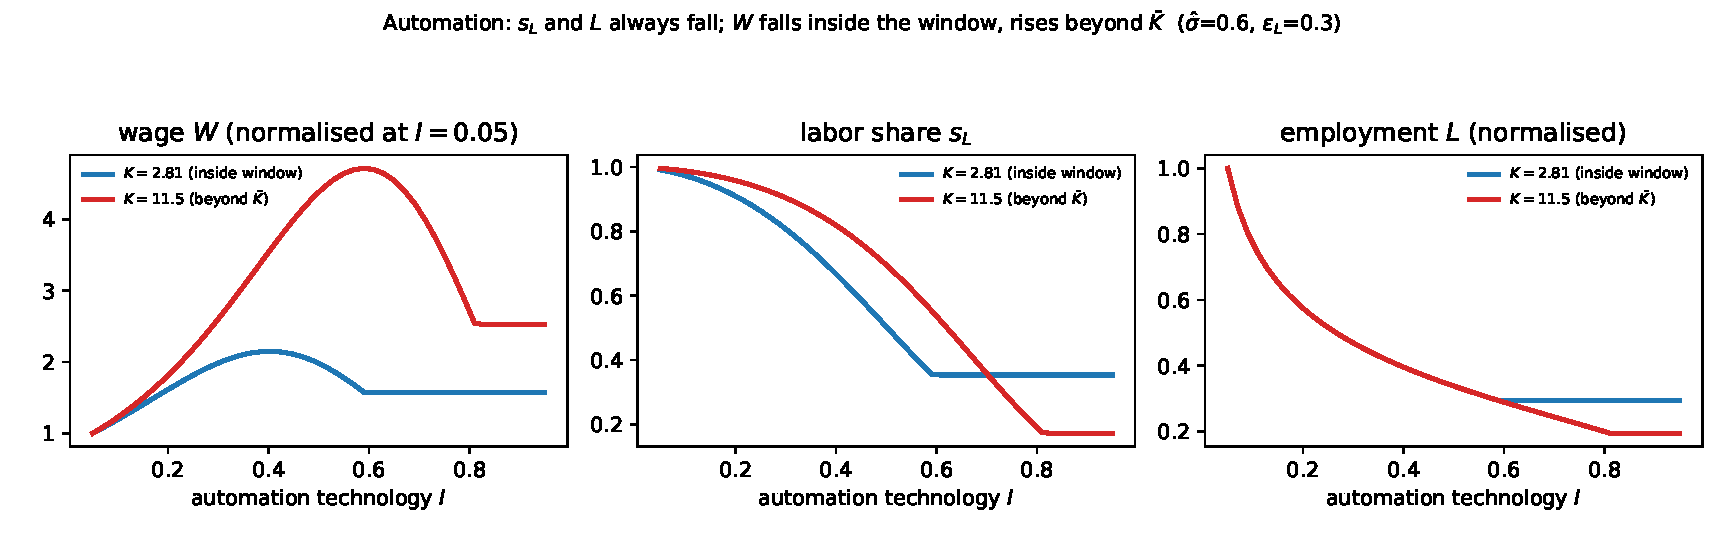
\includegraphics[height=0.8\textheight]{analysis/figures/automation_sweep.pdf}
  \end{center}
\end{frame}

\begin{frame}{3 \textperiodcentered{} $d\ln W/dI$ against $K$: negative inside Assumption 3, positive beyond $\bar K$}
  \begin{center}
    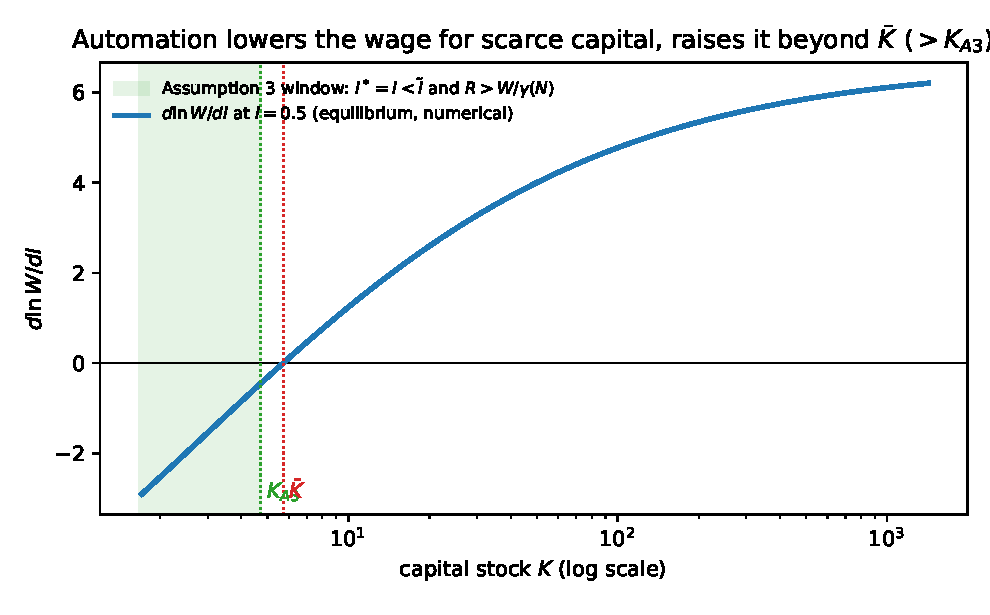
\includegraphics[height=0.8\textheight]{analysis/figures/wage_response_vs_K.pdf}
  \end{center}
\end{frame}

\begin{frame}{3 \textperiodcentered{} Proposition 3 decomposed: productivity effect against displacement effect}
  \begin{center}
    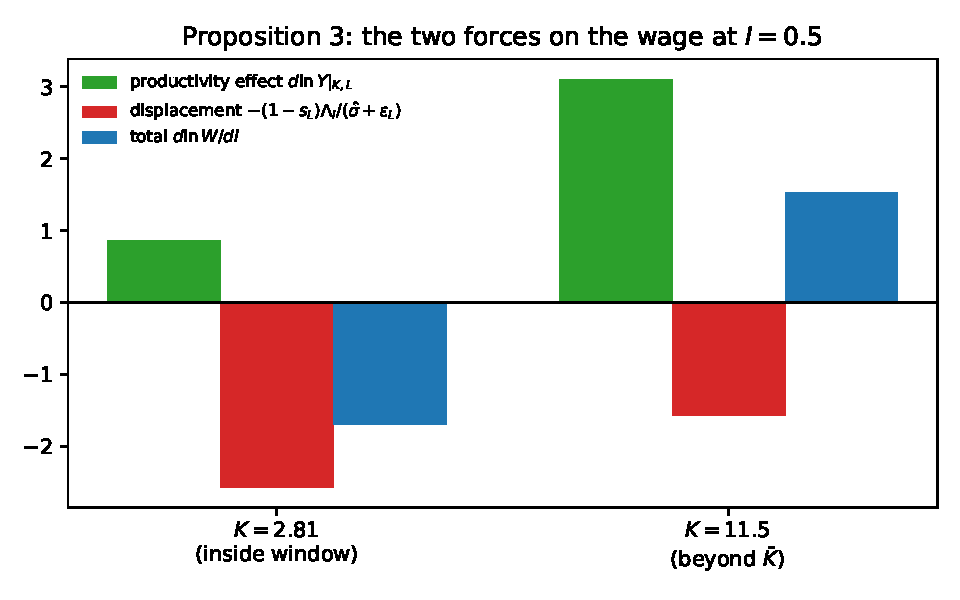
\includegraphics[height=0.8\textheight]{analysis/figures/decomposition.pdf}
  \end{center}
\end{frame}

%================= 4. LEAN ===========================================
\begin{frame}{4 \textperiodcentered{} Lean I: the run, the statement spec, the status}
  \footnotesize
  \textbf{Workflow (AppliedModelingLib, clone at \texttt{2db7d108}).} Pin the June-2017 PDF by SHA-256 $\to$ \texttt{init-spec}
  $\to$ statement spec with 10 targets (PDF-page locators, literal source statements, exact Lean types) $\to$
  \texttt{paper\_contribution.py new --statement-spec} (the scaffold Lean-validates every Spec) $\to$ proofs in
  \texttt{ProofInterface.lean}, extension in \texttt{MainTheorems.lean} $\to$ \texttt{lake build AR18RaceManMachine}
  $\to$ \texttt{check AR18RaceManMachine --fast}. \textbf{Agent:} Claude Code, not Codex (my decision, four hours
  before the deadline; disclosed in \texttt{lean/docs/RUN\_LOG.md}).

  \smallskip
  \textbf{The ten Specs} (\texttt{lean/PaperInterface.lean}), all proved, no \texttt{sorry}: the cost threshold of
  (5)--(6) with $\gamma$ strictly increasing; $I^*=\min\{I,\tilde I\}$; $\Lambda_I,\Lambda_N>0$; Prop.\ 2's three
  signs in the constrained case and $\sigma_{free}>\hat\sigma$; Prop.\ 3's productivity effect $>0$ on both sides
  of $\hat\sigma=1$; automation raises $R$; the wage decomposition as an iff; new tasks raise $W$; Corollary 1's
  marginal products as real derivatives and the labor share $N-I^*$.

  \smallskip
  \textbf{Result:} \texttt{lake build}: Build completed successfully (3313 jobs); \texttt{check --fast}: exit 0.
  \textbf{Status: partially formalized.} The equilibrium map (13) and the derivatives of Prop.\ 2 are taken as
  the paper's displays; the general $\bar K$ is not derived. \textbf{Blocker, stated exactly:} the library root
  \texttt{AppliedModelingLib.olean} does not build on my laptop (disk-bound, 12 h last week), so the paper
  modules import three Mathlib modules instead of \texttt{import Mathlib}, and the spec validation ran under those
  imports instead of \texttt{import AppliedModelingLib}. No library declaration is used.
\end{frame}

\begin{frame}[fragile]{4 \textperiodcentered{} Lean II (required slide): the cost threshold of equations (5)--(6)}
  \scriptsize
  \textbf{Paper (p.\ 10).} $p(i)=\min\{R,W/\gamma(i)\}^{1-\eta}$ for $i\le I$; ``there is a unique threshold
  $\tilde I$ such that $W/R=\gamma(\tilde I)$. For all tasks $i<\tilde I$, we have $R<W/\gamma(i)$''
  (Assumption 1: $\gamma$ strictly increasing).
  \vspace{-2pt}
  \begin{lstlisting}[basicstyle=\ttfamily\tiny]
def paper_cost_thresholdSpec : Prop :=
  ∀ (W R : ℝ) (γ : ℝ → ℝ) (i It : ℝ),
    0 < W → 0 < R → StrictMono γ → (∀ x, 0 < γ x) → γ It = W / R →
      (i < It → R < W / γ i) ∧ (It < i → W / γ i < R)

theorem paper_cost_threshold : paper_cost_thresholdSpec := by
  intro W R γ i It hW hR hmono hpos hIt
  have hγi : 0 < γ i := hpos i
  constructor
  · intro hi
    have h1 : γ i < γ It := hmono hi       -- Assumption 1 does the work
    rw [hIt] at h1                          -- γ i < W / R
    rw [lt_div_iff₀ hR] at h1               -- γ i * R < W
    rw [lt_div_iff₀ hγi]                    -- goal: R * γ i < W
    linarith [mul_comm R (γ i)]
  · intro hi
    have h1 : γ It < γ i := hmono hi
    rw [hIt] at h1; rw [div_lt_iff₀ hR] at h1; rw [div_lt_iff₀ hγi]
    linarith [mul_comm R (γ i)]
  \end{lstlisting}
  \vspace{-4pt}
  \textbf{Reading.} $W,R$ reals, $\gamma$ a real function, $\tilde I$ (\texttt{It}) any real with $\gamma(\tilde I)=W/R$;
  \texttt{StrictMono γ} is Assumption 1 verbatim. The nontrivial step is \texttt{lt\_div\_iff₀}, which moves the positive
  denominator across the inequality; then the claim is linear. Lean verifies the sentence \emph{exactly}, with one
  hypothesis the paper leaves implicit: $\gamma>0$. Uniqueness of $\tilde I$ is not needed by the row.
  \texttt{lake build}: success; \texttt{check --fast}: exit 0.
\end{frame}

\begin{frame}[fragile]{4 \textperiodcentered{} Lean III: the Cobb-Douglas wage response --- the extension that settles the trap}
  \scriptsize
  \textbf{Claim (mine).} With $\ln W=\ln c+\ln s+(1-s)\ln K+(s-1)\ln L$, $s=N-I^*$:
  $\ d\ln W/ds=1/s-\ln K+\ln L$, hence $d\ln W/dI^*=\ln(K/L)-1/(N-I^*)>0\iff e^{1/(N-I^*)}<K/L$.
  \vspace{-2pt}
  \begin{lstlisting}[basicstyle=\ttfamily\tiny]
theorem cobb_douglas_log_wage_deriv (c K L s : ℝ) (hs : 0 < s) :
    HasDerivAt (fun s' : ℝ => Real.log c + Real.log s' + (1 - s') * Real.log K + (s' - 1) * Real.log L)
      (1 / s - Real.log K + Real.log L) s := by
  have h1 : HasDerivAt (fun s' : ℝ => Real.log s') (1 / s) s := by
    simpa [one_div] using Real.hasDerivAt_log hs.ne'
  have h2 : HasDerivAt (fun s' : ℝ => (1 - s') * Real.log K) (-Real.log K) s := by
    have := ((hasDerivAt_id' (x := s)).const_sub 1).mul_const (Real.log K); simpa using this
  have h3 : HasDerivAt (fun s' : ℝ => (s' - 1) * Real.log L) (Real.log L) s := by
    have := ((hasDerivAt_id' (x := s)).sub_const 1).mul_const (Real.log L); simpa using this
  have h := (((hasDerivAt_const s (Real.log c)).add h1).add h2).add h3
  refine h.congr_deriv ?_; ring

theorem cobb_douglas_wage_rises_iff (K L s : ℝ) (hK : 0 < K) (hL : 0 < L) (hs : 0 < s) :
    0 < Real.log (K / L) - 1 / s ↔ Real.exp (1 / s) < K / L := by
  have hKL : 0 < K / L := div_pos hK hL
  rw [sub_pos]; exact Real.lt_log_iff_exp_lt hKL
  \end{lstlisting}
  \vspace{-4pt}
  \textbf{Reading.} The derivative is assembled term by term with \texttt{HasDerivAt} combinators
  (\texttt{Real.hasDerivAt\_log} needs only $s\neq0$); \texttt{congr\_deriv} plus \texttt{ring} matches the paper's
  form. The sign lemma is \texttt{Real.lt\_log\_iff\_exp\_lt}. Since $s=N-I^*$ and $dI^*=-ds$, the wage rises with
  automation iff $K/L>e^{1/(N-I^*)}$: \textbf{abundant capital}. Under Assumption 3, $K/L<(1-s)/s<e^{1/s}$, so
  the printed ``increases the wage when $K<\bar K$'' cannot be right for this case; the numerics agree for $\hat\sigma\neq1$.
\end{frame}

%================= 5. DONDE NO LE CREI A LA IA =======================
\begin{frame}{5 \textperiodcentered{} Where I did not believe the AI --- and where I did not believe the paper}
  \begin{columns}[T]
    \column{0.30\textwidth}
      \IfFileExists{hand/hand-derivation-part1.png}{%
        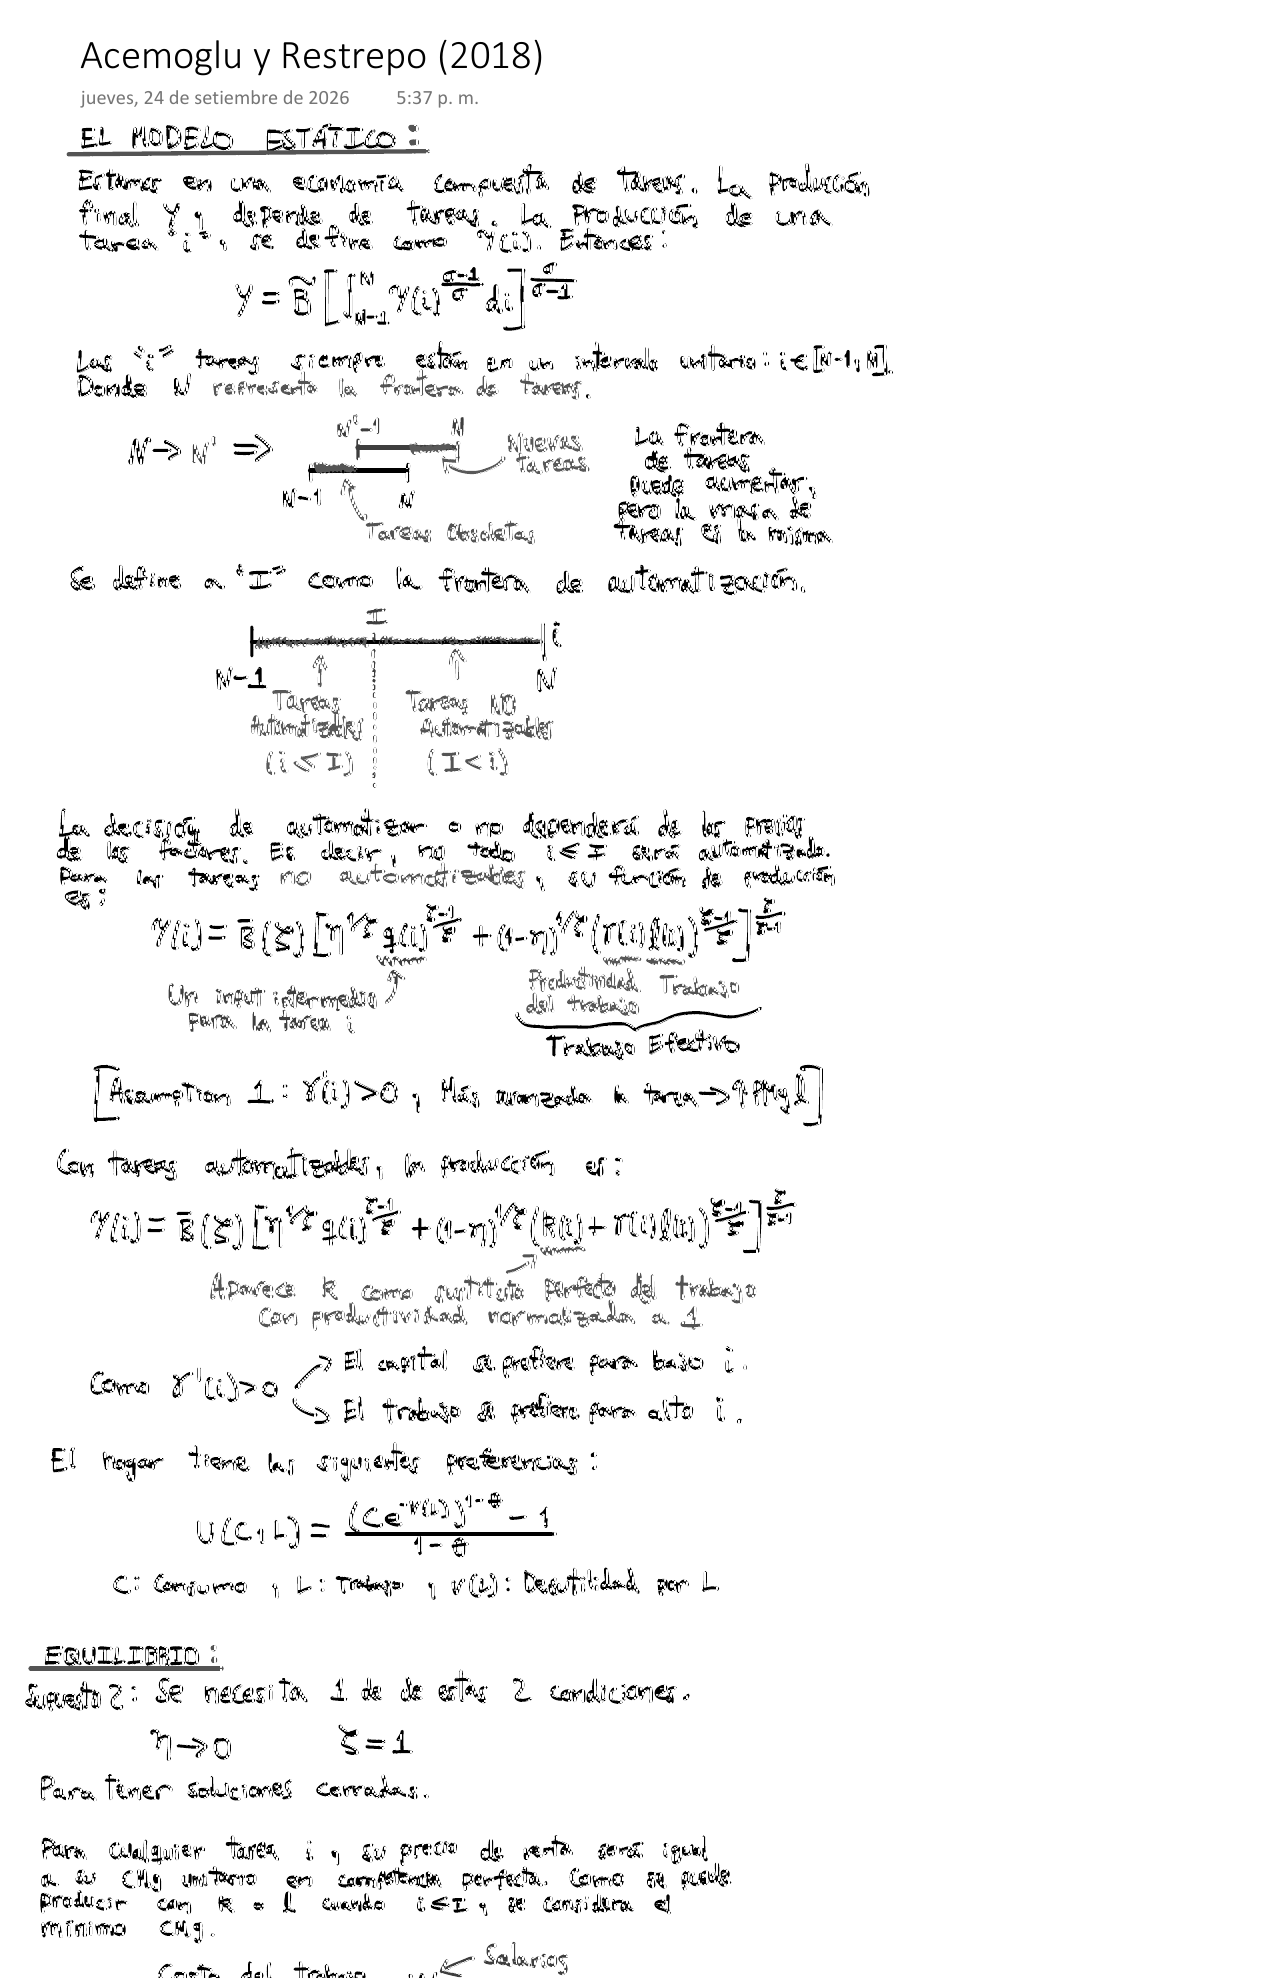
\includegraphics[height=0.66\textheight]{hand/hand-derivation-part1.png}}{%
        \IfFileExists{hand/hand-derivation.pdf}{%
          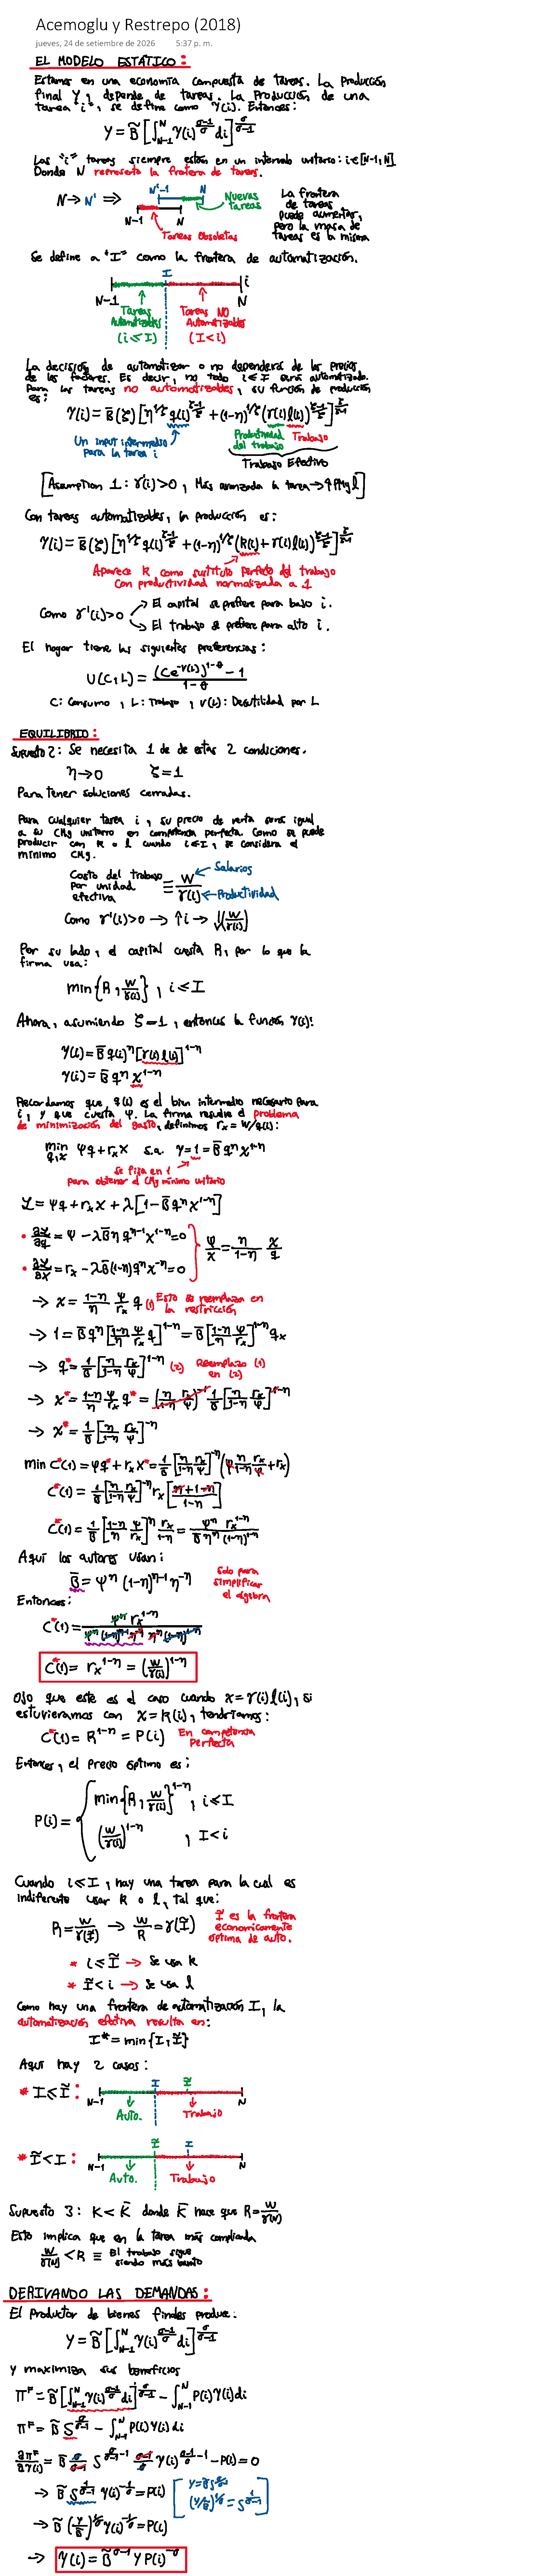
\includegraphics[page=1,height=0.66\textheight]{hand/hand-derivation.pdf}}{%
          \fbox{\parbox{0.8\linewidth}{\centering\scriptsize hand derivation\\ \texttt{hand/}}}}}
      \\[2pt]{\scriptsize Hand derivation: the threshold and the Cobb-Douglas wage. Full pages in the backup.}
    \column{0.68\textwidth}\footnotesize
      \textbf{Claim 1 (the flat answer):} ``automation lowers wages and the labor share.'' Props.\ 2--3: the labor
      share always falls when technology binds; the wage rises iff productivity beats displacement, and does not
      move in the cost-minimising regime. \textbf{Verdict: half right.}

      \smallskip
      \textbf{Claim 2 (my first numerics):} I wrote $W/R=\omega K/L$; Prop.\ 2's $d\ln(W/R)/dI=d\ln\omega/dI$ then
      failed by $(1-\varepsilon_L)$. The paper's $\omega=W/(RK)$ gives $W/R=\omega K$; fixed, the numerical derivative
      matches Prop.\ 3's formula to four decimals. \textbf{Verdict: I was wrong; the check caught it.}

      \smallskip
      \textbf{Claim 3 (the paper):} ``there exists $\bar K>\underline K$ such that an increase in $I$ increases the
      wage when $K<\bar K$ and reduces it when $K>\bar K$.'' By hand and in Lean, Cobb-Douglas gives
      $d\ln W/dI^*=\ln(K/L)-1/(N-I^*)$: the wage rises for \emph{large} $K$, so with $\bar K>\underline K$ it always
      falls inside Assumption 3; the $\hat\sigma=0.6$ numerics and the paper's own intuition (cost savings
      $W/\gamma(I^*)-R$) agree. \textbf{Verdict: the two inequalities are printed the wrong way round} (AER text not checked).

      \smallskip
      \textbf{Claim 4 (Lean pushed back):} the productivity term divides by $1-\hat\sigma$; the sign proof needs
      $\hat\sigma<1$ and $\hat\sigma>1$ separately and excludes $\hat\sigma=1$ --- the Cobb-Douglas limit the paper takes silently.
  \end{columns}
\end{frame}

\begin{frame}{5 \textperiodcentered{} What to carry away}
  \footnotesize
  \begin{itemize}
    \item \textbf{Two forces, not one.} Automation \emph{displaces} (fewer tasks for labor: $W/R$, $s_L$, $L$
      fall) but also raises productivity; new tasks \emph{reinstate} labor. The race is between $I$ and $N$.
    \item \textbf{The wage condition.} Automation raises the wage iff the cost saving on the marginal task,
      $W/\gamma(I^*)-R$, outweighs $(1-s_L)\Lambda_I/(\hat\sigma+\varepsilon_L)$ --- i.e.\ when capital is abundant
      (Cobb-Douglas: $K/L>e^{1/(N-I^*)}$). Under the paper's Assumption 3 it falls.
    \item \textbf{Regime matters.} If technology does not bind ($I^*=\tilde I<I$), better automation technology
      changes nothing; only $N$ moves prices.
    \item \textbf{Lean.} Ten rows proved exactly from the displays; the equilibrium map and the general $\bar K$ are
      the declared boundary; the extension proves the closed-form threshold and exposes the reversed inequality.
    \item \textbf{Versions.} NBER June 2017 (course PDF) read and pinned; AER 2018 reverses the title; the page
      numbers here are the PDF's.
  \end{itemize}
\end{frame}

%================= BACKUP =============================================
\begin{frame}{B1 \textperiodcentered{} New tasks: $W$ and $s_L$ always rise (reinstatement)}
  \begin{center}
    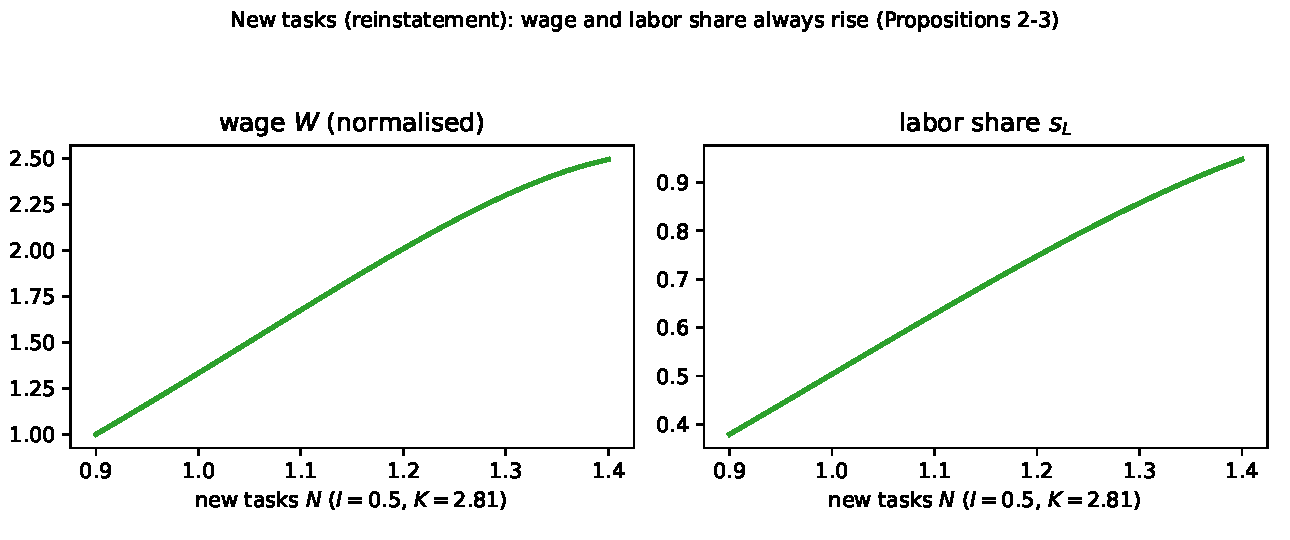
\includegraphics[height=0.8\textheight]{analysis/figures/new_tasks_sweep.pdf}
  \end{center}
\end{frame}

\begin{frame}{B2 \textperiodcentered{} Hand derivation}
  \begin{center}
    \IfFileExists{hand/hand-derivation-part1.png}{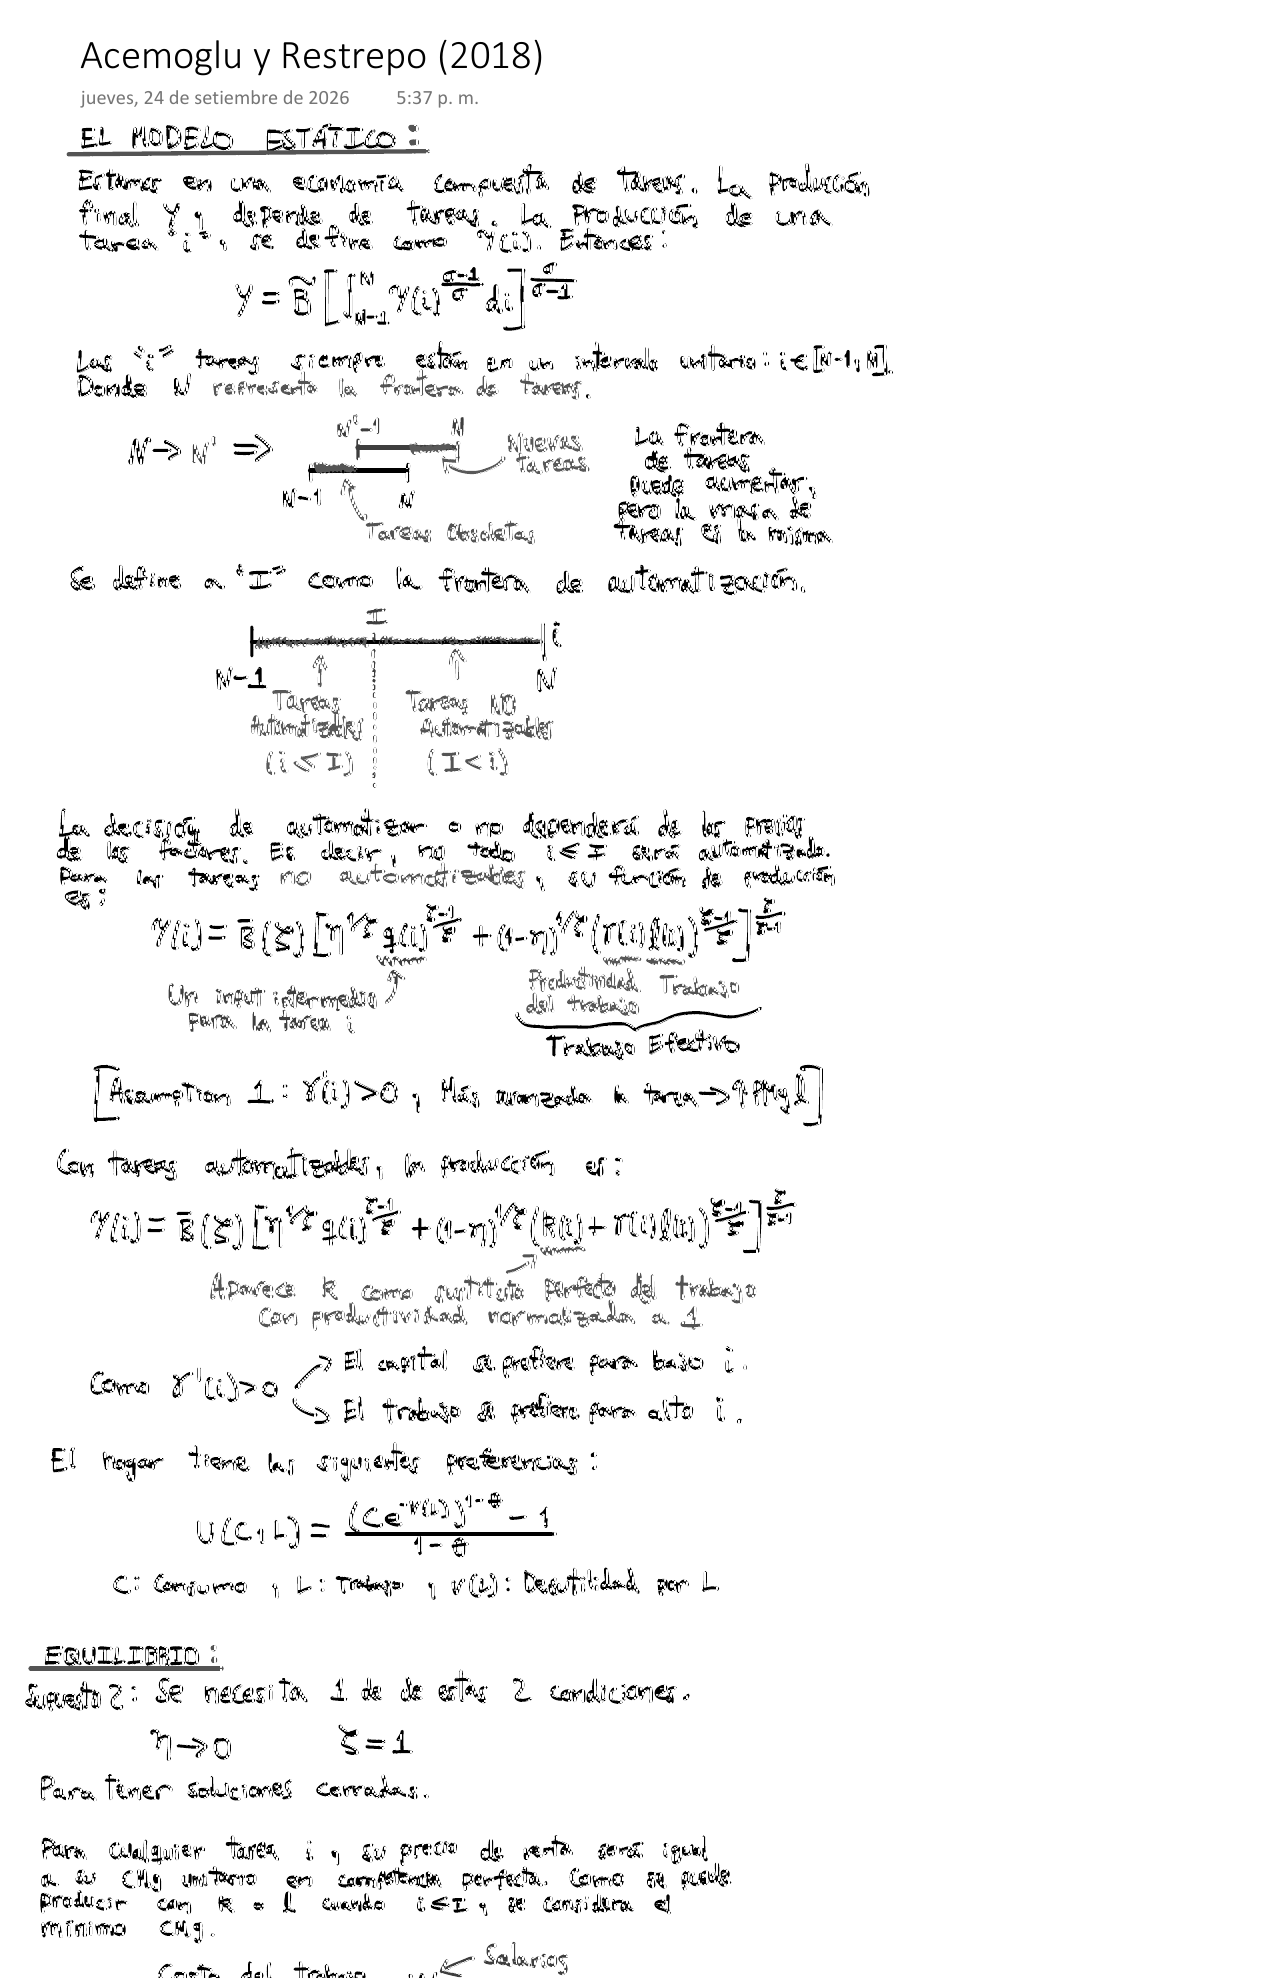
\includegraphics[height=0.84\textheight]{hand/hand-derivation-part1.png}}{%
      \IfFileExists{hand/hand-derivation.pdf}{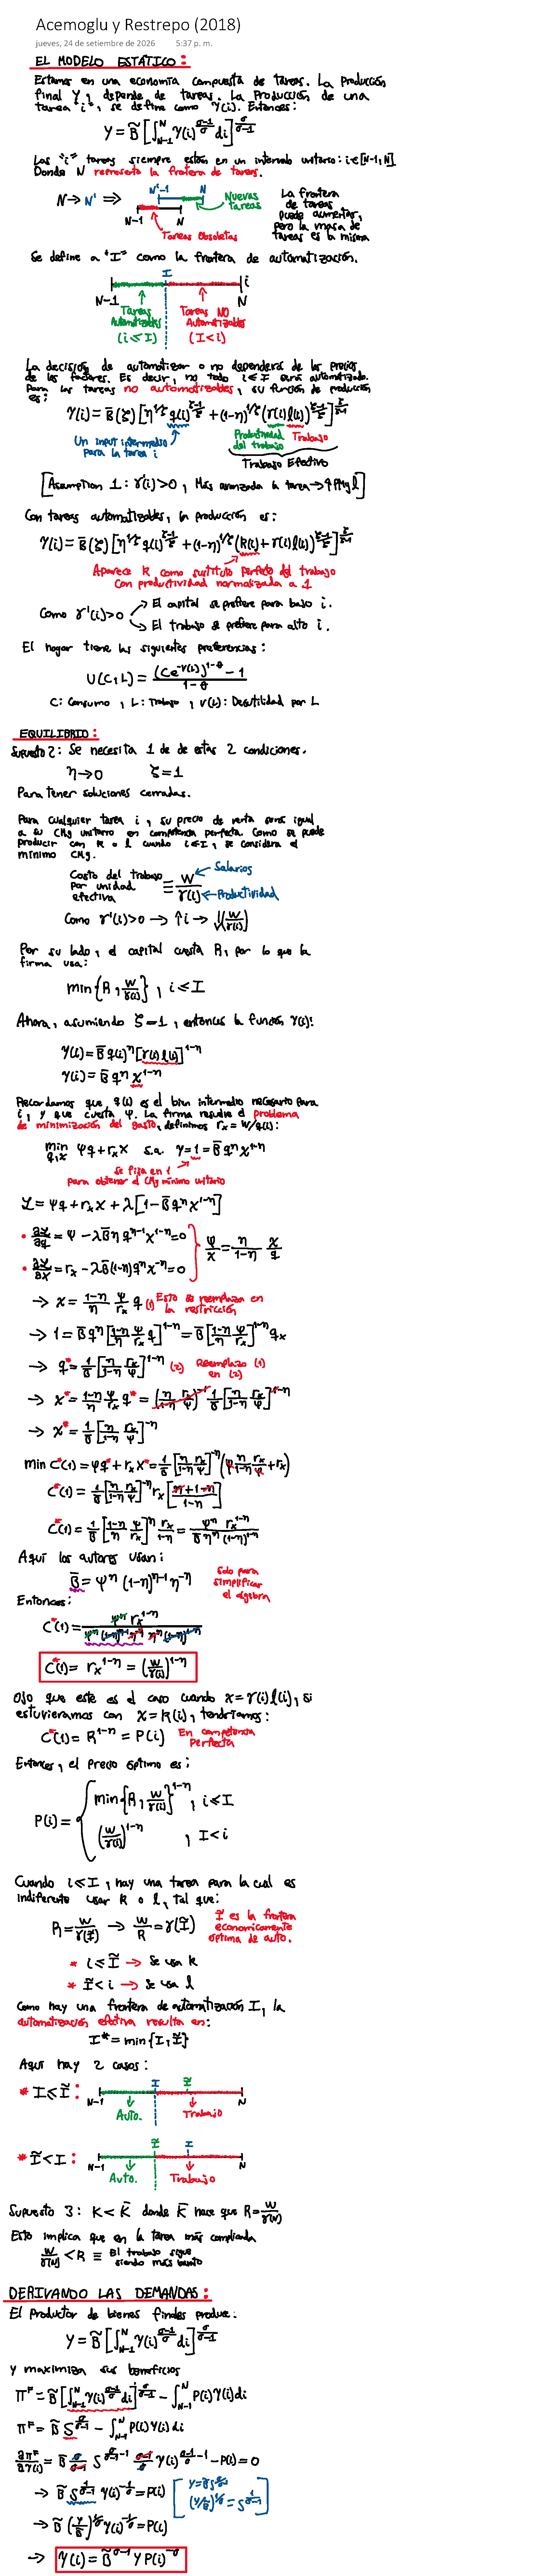
\includegraphics[page=1,height=0.84\textheight]{hand/hand-derivation.pdf}}{%
        \fbox{\parbox{0.6\linewidth}{\centering hand derivation (\texttt{hand/})}}}}
  \end{center}
\end{frame}

\begin{frame}[fragile]{B3 \textperiodcentered{} Lean IV: Proposition 3's productivity effect on both sides of $\hat\sigma=1$}
  \scriptsize
  \begin{lstlisting}[basicstyle=\ttfamily\tiny]
def paper_prop3_productivity_effect_positiveSpec : Prop :=
  ∀ Wg R σh : ℝ, 0 < R → R < Wg → σh ≠ 1 →
    0 < (Wg ^ (1 - σh) - R ^ (1 - σh)) / (1 - σh)

theorem paper_prop3_productivity_effect_positive : paper_prop3_productivity_effect_positiveSpec := by
  intro Wg R σh hR hlt hne
  rcases lt_or_gt_of_ne hne with hlt1 | hgt1
  · have hexp : 0 < 1 - σh := by linarith
    have h : R ^ (1 - σh) < Wg ^ (1 - σh) := Real.rpow_lt_rpow hR.le hlt hexp
    exact div_pos (by linarith) hexp
  · have hexp : 1 - σh < 0 := by linarith
    have h : Wg ^ (1 - σh) < R ^ (1 - σh) := Real.rpow_lt_rpow_of_neg hR hlt hexp
    exact div_pos_of_neg_of_neg (by linarith) hexp

def paper_prop3_wage_decompositionSpec : Prop :=
  ∀ P sL ΛI σh εL dI : ℝ,
    0 < P - (1 - sL) * ((1 / (σh + εL)) * ΛI * dI) ↔
      (1 - sL) * ((1 / (σh + εL)) * ΛI * dI) < P
  \end{lstlisting}
  \textbf{Reading.} \texttt{Wg} is $W/\gamma(I^*)$ and \texttt{R} the rental rate; the hypothesis \texttt{R < Wg} is the
  constrained case of Proposition 3. For $\hat\sigma<1$ the real power is increasing and both numerator and
  denominator are positive; for $\hat\sigma>1$ both are negative. The decomposition row states the wage sign as an
  equivalence over the paper's display: productivity effect $P$ against displacement.
\end{frame}

\end{document}
